\documentclass[../../main/main.tex]{subfiles}
\begin{document}

\section{Monotone Strategy Proofs}
\label{sec:monotone_proofs}

This appendix provides the detailed proofs regarding monotone calling strategies and their relationship to the uniqueness of the Nash equilibrium in LCP.

\subsection{Monotone Strategies and Weak Dominance}

\begin{lemma}
    \label{lem:monotone_dominated}
    If a calling strategy violates the first monotonicity condition for a nonzero-measure set of hands for any bet size $s$, it is weakly dominated. Specifically, if there exists $s$ and measurable sets $A, B \subseteq [0, 1]$ such that:
    \begin{enumerate}
        \item The caller calls $s$ with hands in $A$
        \item The caller folds $s$ with hands in $B$
        \item $\sup A \leq \inf B$
        \item $A$ and $B$ have positive measure
    \end{enumerate}
    then the strategy is weakly dominated.
\end{lemma}

\begin{proof}
    Let $\sigma_C$ be the non-monotone strategy described above. Since $A$ and $B$ are nonzero-measure, there exist subsets $A' \subseteq A$ and $B' \subseteq B$ such that:
    \begin{enumerate}
        \item $A'$ and $B'$ have positive measure
        \item $|A'| = |B'|$
    \end{enumerate}
    Where $|A|$ and $|B|$ denote the Lebesgue measure of $A$ and $B$ (see Figure \ref{fig:strategy_improvement}).

    \begin{figure}[h]
        \centering
        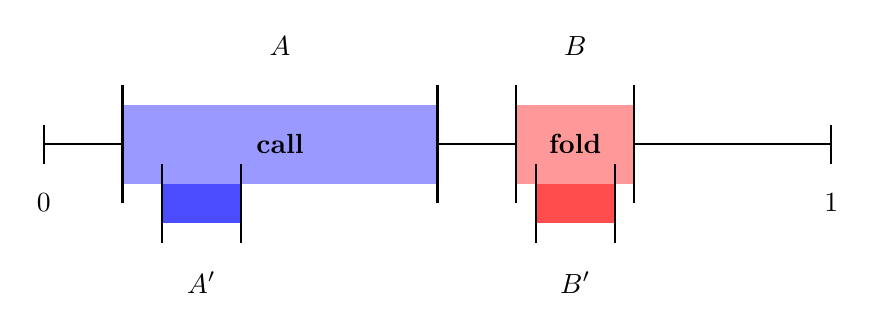
\begin{tikzpicture}[scale=5]
            % Number line from 0 to 1
            \draw[thick] (0,0) -- (2,0);

            % Tick marks at 0 and 1
            \draw[thick] (0, -0.05) -- (0, 0.05);
            \draw[thick] (2, -0.05) -- (2, 0.05);

            % Endpoint labels
            \node[below] at (0, -0.1) {$0$};
            \node[below] at (2, -0.1) {$1$};

            % Set A (calling hands) - blue
            \fill[blue!40] (0.2, -0.1) rectangle (1.0, 0.1);
            \draw[thick] (0.2, -0.15) -- (0.2, 0.15);
            \draw[thick] (1.0, -0.15) -- (1.0, 0.15);
            \node[above] at (0.6, 0.2) {$A$};
            \node at (0.6, 0) {\textbf{call}};

            % Set B (folding hands) - red
            \fill[red!40] (1.2, -0.1) rectangle (1.5, 0.1);
            \draw[thick] (1.2, -0.15) -- (1.2, 0.15);
            \draw[thick] (1.5, -0.15) -- (1.5, 0.15);
            \node[above] at (1.35, 0.2) {$B$};
            \node at (1.35, 0) {\textbf{fold}};

            % Set A' (subset of A) - darker blue
            \fill[blue!70] (0.3, -0.2) rectangle (0.5, -0.1);
            \draw[thick] (0.3, -0.25) -- (0.3, -0.05);
            \draw[thick] (0.5, -0.25) -- (0.5, -0.05);
            \node[below] at (0.4, -0.3) {$A'$};

            % Set B' (subset of B) - darker red
            \fill[red!70] (1.25, -0.2) rectangle (1.45, -0.1);
            \draw[thick] (1.25, -0.25) -- (1.25, -0.05);
            \draw[thick] (1.45, -0.25) -- (1.45, -0.05);
            \node[below] at (1.35, -0.3) {$B'$};

        \end{tikzpicture}
        \caption{A simple case of sets $A$ and $B$ which violate monotonicity ($\sup A \leq \inf B$). We can find equal-measure subsets $A' \subseteq A$ and $B' \subseteq B$ to swap actions, improving the strategy.}
        \label{fig:strategy_improvement}
    \end{figure}

    The existence of such subsets follows from a fundamental property of nonatomic measures: since the uniform distribution on $[0,1]$ is nonatomic (no single point has positive probability), for any two measurable sets with positive measure, we can always find measurable subsets of equal measure\cite{Sierpinski1922}. This property allows us to construct the strategy improvement described below.

    Let $\sigma_C'$ be the strategy which switches the actions for $A'$ and $B'$, i.e. calls with $B'$ and folds with $A'$ (and behaves identically for all other bet sizes). We now analyze how this change affects the caller's performance against any betting strategy.

    Against a bet of size $s$, the key improvement occurs in two scenarios:
    \begin{enumerate}
        \item When $y \in B'$ and $x \in A'$: $\sigma_C$ folds while $\sigma_C'$ calls and wins (since $x \in A$ and $y \in B$ with $\sup A \leq \inf B$)
        \item When $y \in A'$ and $x \in B'$: $\sigma_C$ calls and loses while $\sigma_C'$ folds (avoiding the loss)
    \end{enumerate}

    For all other cases, $\sigma_C$ and $\sigma_C'$ behave identically, so $\sigma_C'$ is weakly better than $\sigma_C$ against every betting strategy.

    To show that $\sigma_C$ is strictly dominated, consider a betting strategy which always bets $s$. Against this strategy, both scenarios above occur with positive probability (since $A'$ and $B'$ have positive measure), so $\sigma_C'$ is strictly better than $\sigma_C$. Thus, $\sigma_C$ is weakly dominated.
\end{proof}

\subsection{Monotone-Admissibility and Uniqueness}

The second monotonicity condition - that the caller must be more willing to call smaller bets - cannot be derived from dominance arguments alone. However, it plays a crucial role in selecting among the infinite class of Nash equilibria that differ only in how the bettor sizes their bluffs.

\textbf{Motivation:} From a poker player's perspective, this condition aligns with intuition about pot odds: a larger bet is riskier and should require a stronger hand to call. While violating this condition is not strictly dominated (and indeed occurs in real poker when players perceive larger bets as bluffs), it leads to exploitable calling strategies.

If the caller violates this condition by calling less aggressively against smaller bets, the bettor can exploit this by taking smaller risks for higher returns. A monotone calling strategy is therefore less exploitable. Imposing this condition restricts the strategy space in a way that yields a unique Nash equilibrium.

\begin{definition}[Monotone-Admissible Strategy]
    A betting strategy $\sigma_B$ is \textit{monotone-admissible} if it is admissible in LCP against the set of monotone calling strategies. More explicitly, $\sigma_B$ is monotone-admissible if there does not exist a betting strategy $\sigma_B'$ such that both of the following hold:
    \begin{enumerate}
        \item $\pi_B(\sigma_B',\sigma_C) \geq \pi_B(\sigma_B,\sigma_C)$ for all monotone calling strategies $\sigma_C$
        \item $\pi_B(\sigma_B',\sigma_C) > \pi_B(\sigma_B,\sigma_C)$ for at least one monotone calling strategy $\sigma_C$
    \end{enumerate}
\end{definition}

\textbf{Application to LCP:} This definition is particularly useful in distinguishing bettor strategies which differ only in how they bluff. The hand strength of a bluff is irrelevant when the caller plays optimally, since the caller will never call with a hand weaker than any bluff. However, if the caller deviates to a suboptimal but still monotone strategy, then the bettor's bluffing hand strength becomes important.

Specifically, if the caller becomes too loose (calling too often with weak hands), then the bettor wins some pots "accidentally" when they make their smallest bluffs with their strongest bluffing hands. This is where monotone-admissibility differentiates between equilibria: the unique monotone-admissible equilibrium has the bettor bluffing larger with weaker hands and bluffing smaller with stronger hands, which is optimal against all monotone deviations by the caller.

\end{document}
